\section{Introduction}
\label{sec:Introduction}
\subsection{Lattices}
\label{subsec:Introduction-Lattices}
A lattice $\calC$ is a poset \st for any pair $(a,b) \in \calC$, the supremum $a \land b$, and infimum $a \lor b$ exist. We extend this to a complete lattice, which has the requirement that for any subset $\calD \subseteq \calC$ the supremum $\bigvee \calD$ and infimum $\bigwedge \calD$ exist. 

\subsubsection{Supremum and infimum} 
\label{subsubsec:Introduction-Lattices-Supremum_and_Infimum}
The supremum of two elements is defined as the \textit{least upper bound} of those two elements. We can obviously extend this over more than two elements. Given the set $S = \{1,2,3,4,5\}$, where $S \subset \mathbb{N}$. The supremum, $\bigvee S = 5$; similarly, the infimum $\bigwedge S = 1$.  

\begin{figure}[h]
    \centering
    \begin{tikzpicture}[node distance=1cm]
        \node (top) at (0,2) {$1$};
        \node (a) at (-1,0) {$a$};
        \node (b) at (1,0) {$b$};
        \node (c) at (1, -1) {$c$};
        \node (d) at (-1, -1) {$d$};
        \node (bottom) at (0,-3) {$0$};
        
        \draw (top) -- (a);
        \draw (top) -- (b);
        \draw (a) -- (c);
        \draw (b) -- (c);
        \draw (a) -- (d);
        \draw (c) -- (bottom);
        \draw (d) -- (bottom);
    \end{tikzpicture}
    \caption{$d \lor c = a$, $b\land a = c$}
    \label{fig:Demostration of Supremum and Infimum in Lattices }
\end{figure}

When we are talking about lattices (or Hasse diagrams in general), we can refer to the supremum and infimum as the \textit{meet} and \textit{join}. Refer to \ref{subsec:Introduction-The_Basic_Theorem} for more pertinent discusison regarding lattices.

We also have infimum (supremum) satisfying the following 
\begin{itemize}
    \item $x \land y = y \lor x$ (commutativity) 
    \item $x \lor (y \lor z) = (x \lor y) \lor z$ (associativity)
    \item $x \lor x$ (idempotency - but arguably, reflexivity)
\end{itemize}

We use these later on to show that any finite lattice is a complete lattice. 

There are also the following interesting properties: 
\begin{itemize}
    \item $a \lor 0 = a$ 
    \item $a \leq b \implies a \lor b = b$\footnote{This is useful because it enables to move from orders (posets) to lattices}
\end{itemize}

\subsection{Formal Contexts}
\label{subsec:Introduction-Formal_Contexts}
A Formal Context is a triple $\langle G, M, I \rangle$ where $G$ refers to a set of objects, $M$ to a set of properties, and $I$ an incidence relation over $G\times M$. 

We have derivation operators $A'$ and $B'$; for $A'$, where $A \subseteq G$, the derivation operator tells us which properties belong to the objects in $A$, the dual holds for properties and their objects. \textbf{Formally}, 

\begin{definition}
    \[ A' := \left\{m \in M \,|\, \forall g \in A, gIm\right\} \]
    \[ B' := \left\{g \in G \,|\, \forall m \in B, gIm\right\} \]
\end{definition}

We also have closure operators, $A''$, which works intuitively by applying the derivation operator on $A$ ($B$), which yields a set of properties. Then applying it again on $A'$ ($B'$), which yields back a set of objects (properties). 

\begin{proposition}
    For subsets $A, B\subseteq G$ (defined dually for properties $C,D \subseteq M$), we have
    \begin{itemize}
        \item[a.] $A \subseteq B \implies B' \subseteq A'$ 
        \item[b.] $A \subseteq A''$ 
        \item[c.] $A' = A'''$
    \end{itemize}
\end{proposition}

For more natural discussion, \textit{a} describes the behaviour that if we have two sets of objects $A$ and $B$, where $A \subseteq B$; then it follows that objects in $A$ will have at \textit{least} all the properties of objects in $B$. 

\subsection{Formal Concepts}
\label{subsec:Introduction-Formal_Concepts}

\textit{Presume we are working with a formal context $\langle G, M, I \rangle$.}
\begin{definition}
    
    $(A,B)$ is a \textit{\textbf{formal concept}} of our formal context \textit{iff}    $A \subseteq G$, $B \subseteq M$, $A' = B$, and $B' = A$ 
\end{definition}

$A$ is called the \textbf{extent}, and $B$ is called the \textbf{intent}. We can refer to the set of all formal concepts of a formal context as a $\calB (G, M, I)$.

\subsection{Concept Hierarchies}
\label{subsec:Introduction-Concept_Hierarchies}

When we think about concepts, we typically think of them in a structure (something like a taxonomy, or ontology). That is, we think of \textit{sub} and \textit{super} concepts. For example, Dog is a subconcept of Mammal; and so is Cat. However, Dog and Cat are not sub nor superconcepts of one another (so, in some sense we have a partial order here). Formal Concepts have the same idea. 

\begin{definition}
    Let $(A_1, B_1)$ and $(A_2, B_2)$ be formal concepts of some $\calB(G,M,I)$. We say that $(A_1,B_1)$ is a \textbf{subconcept} of $(A_2,B_2)$ (equivalently, $(A_2,B_2)$ is a \textbf{superconcept} of $(A_1, B_1)$) and use the $\leq$ sign to express this. Thus we have 
    
    \[(A_1, B_1)\leq (A_2, B_2) :\iff A_1 \subseteq A_2 \space (\iff B_2 \subseteq B_1).\]
\end{definition}

\subsection{The Basic Theorem}
\label{subsec:Introduction-The_Basic_Theorem}
\subsubsection{I} 
\label{subsec:Introduction-The_basic_Theorem-I}
The first part of the Basic Theorem tells us that given some formal concept $(G,M,I)$, the concept lattice of $\calB(G,M,I)$ is a complete lattice. So, constructing a lattice from a formal context, will always result in a complete lattice. 

\textbf{From $\calB(G,M,I)$}, let $\{(A_t, B_t) | t\in T\} \subseteq \calB (G,M,I)$ be some arbitrary subset of formal concepts. We can then define the supremum and infimum of this subset as: 
\[ \bigvee_{t\in T} (A_t, B_t) := \Big( (\bigcup_{t\in T} A_t)'', (\bigcap_{t\in T}B_t) \Big)\] 
\[ \bigwedge_{t\in T} (A_t, B_t) := \Big( (\bigcap_{t\in T} A_t), (\bigcup_{t\in T}B_t)'' \Big)\] 

Now, we want to show that there is some complete lattice $\mathcal{V}$ that is isomorphic to the concept lattice given by $\calB(G,M,I)$.
\begin{center}
    \begin{tabular}{c|cccccc}
        & Fur & Feathers & Scales & Lives on Land & Lays Eggs & Cold-Blooded \\ \hline
        Mammals     & $\times$   &       &         &  $\times$ & &          \\
        Birds       &     & $\times$     &         & $\times$   & $\times$ &          \\
        Reptiles    &     &       & $\times$       & $\times$   & $\times$ & $\times$        \\
        Amphibians  &     &       & $\times$       & $\times$   & $\times$ & $\times$        \\
        Fish        &     &       & $\times$       &     &   & $\times$        \\
    \end{tabular}
\end{center}

Suppose we are interested in Mammals and Birds, $\{Mammals\}' = \{Fur, Lives on Land\}$; $\{Mammals\}'' = \{Mammals\}$. $\{Birds\}' = \{Feathers, Lives on Land, Lays Eggs\}; \{Birds\}'' = \{Birds\}$.

Using the basic theorem from above, we can determine the supremum and infimum of our set of concepts. We have the set of concepts from above, lets call this $ S := (A_t, B_t$. We can calculate $\bigvee S$ by 
\[\Big(\bigcup_{t\in T} A_t)'', \bigcap_{t\in T} B_t\Big)\] 
\[\Big(\{Mammals, Birds\}'', \{Lives on Land\} \Big)\] 
\[\Big( \{Mammals, Birds, Amphibians, Reptiles\}, \{Lives on Land\}\Big)\] 

Dually, we can find the infimum $\bigwedge S$, given as: (which is the bottom element) 
\[\Big(\bigcap_{t\in T}A_t, (\bigcup_{t\in T}B_t)'' \Big) \]
\[\Big(\emptyset, (\{Fur, Feathers, Lives on Land, Lays Eggs\})\Big) \]
\[\Big(\emptyset, \emptyset \Big) \]

The first part of the Basic Theorem, which we have just gone through, shows that for the concept lattice of a given formal context, $\calB (G,M,I)$, we have an infimum and supremum for any arbitrary subset of concepts. This is just our definition of a complete lattice - so we have that any formal context has a complete lattice. 

\subsubsection{II} 
\label{subsec:Introduction-The_basic_Theorem-II}
The second part of the basic theorem tells us that every complete lattice is \textit{isomorphic} to a concept lattice. That is, given a complete lattice $(\mathcal{L}, \leq)$, we can find some $\calB (G,M,I)$ that is isomorphic to $\mathcal{L}$. 

\begin{example}
    \begin{figure}[h]
        \centering
        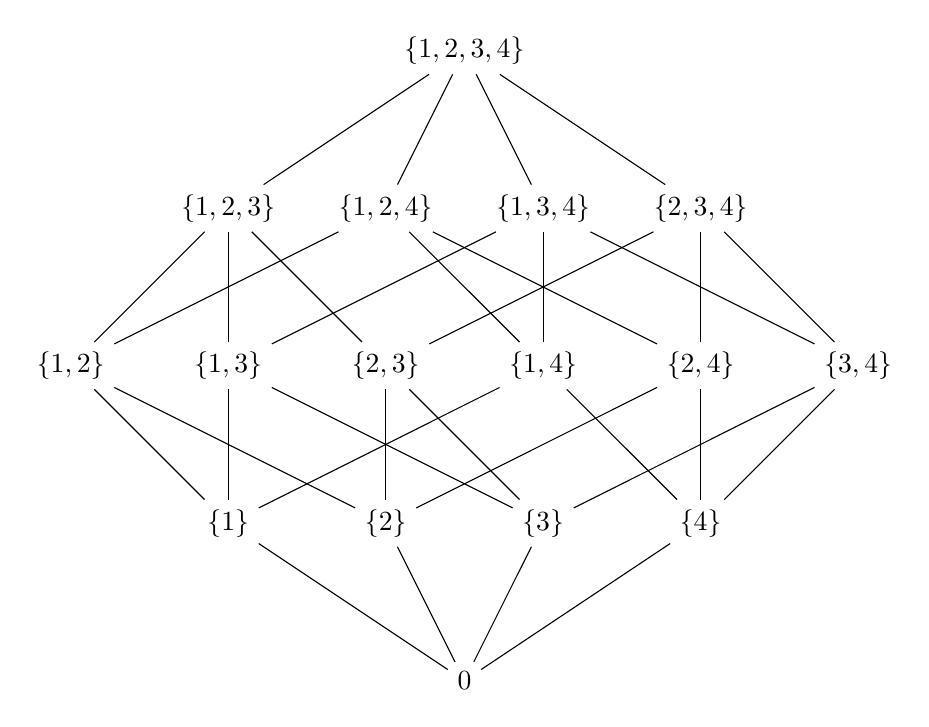
\begin{tikzpicture}[node distance=4cm]
            \node (top) at (0,2) {$\{1,2,3,4\}$};
            \node (a) at (-3,0) {$\{1,2,3\}$};
            \node (b) at (-1,0) {$\{1,2,4\}$};
            \node (c) at (1,0) {$\{1,3,4\}$};
            \node (d) at (3,0) {$\{2,3,4\}$};

            \node (e) at (-5, -2) {$\{1,2\}$};
            \node (f) at (-3, -2) {$\{1,3\}$};
            \node (g) at (1, -2) {$\{1,4\}$};
            \node (h) at (-1, -2) {$\{2,3\}$};
            \node (i) at (3, -2) {$\{2,4\}$};
            \node (j) at (5, -2) {$\{3,4\}$};

            \node (k) at (-3, -4) {$\{1\}$};
            \node (l) at (-1, -4) {$\{2\}$};
            \node (m) at (1, -4) {$\{3\}$};
            \node (n) at (3, -4) {$\{4\}$};

            \node (bottom) at (0,-6) {$0$};

            \draw (top) -- (a);
            \draw (top) -- (b);
            \draw (top) -- (c);
            \draw (top) -- (d);
            \draw (e) -- (a);
            \draw (e) -- (b); 
            \draw (f) -- (a); 
            \draw (f) -- (c); 
            \draw (g) -- (b); 
            \draw (g) -- (c); 
            \draw (h) -- (a); 
            \draw (h) -- (d);
            \draw (i) -- (b); 
            \draw (i) -- (d); 
            \draw (j) -- (c); 
            \draw (j) -- (d);
            \draw (k) -- (e); 
            \draw (k) -- (f); 
            \draw (k) -- (g); 
            \draw (l) -- (e); 
            \draw (l) -- (h); 
            \draw (l) -- (i); 
            \draw (m) -- (f); 
            \draw (m) -- (h);
            \draw (m) -- (j);
            \draw (n) -- (g);
            \draw (n) -- (i); 
            \draw (n) -- (j);
            \draw (k) -- (bottom);
            \draw (l) -- (bottom);
            \draw (m) -- (bottom);
            \draw (n) -- (bottom);
        \end{tikzpicture}
        \caption{Example of a complete lattice of ($\{1,2,3,4\}, \subseteq$)}
        \label{fig:Demostration of Supremum and Infimum in Lattices }
    \end{figure}
\end{example}

This is a complete lattice (it is finite, so it is complete); we can find a relatively simply formal context, which is isomorphic to the lattice: we need two sets, the set of supremum-irreducible elements, and the set of infimum-irreducible elements. For small lattices, we can do this via inspection - the supremum-irreducible (infimum-irreducible) elements are those which which only have a single line below (above) the element. 

Thus, our supremum-irreducible set is $\{1,2,3,4\}$; 

and our infimum-irreducible set is $\{\{1,2,3\}, \{1,2,4\}, \{1,3,4\}, \{2,3,4\}\}$. 

The supremum-irreducible set represents the objects, and infimum-irreducible set represents the properties. The reason for this is inuitive: we start bottom-up with our maximally sub-concepts (remember, the distinction between properties and objects is a modelling problem), these basic elements are the ones which supremum-irreducible, i.e. they cannot be written as a super-concept of some other elements. Conversely, our infimum-irreducible elements are the most general (other than $\top$) elements of our lattice, they cannot be written as the sub-concepts of elements.\footnote{We can of course write a  infimum-irreducible element $e$ as $e \lor \top$, but this is not useful.} 

\begin{table}[h]
    \centering
    \caption{The formal context for \ref{fig:Demostration of Supremum and Infimum in Lattices }}
    \begin{tabular}{c|cccc} 
        & $\{1,2,3\}$ & $\{1,2,4\}$ & $\{1,3,4\}$ & $\{2,3,4\}$ \\ \hline
        $1$ & $\times$ & $\times$ & $\times$ & \\ 
        $2$ & $\times$ & $\times$ & & $\times$ \\ 
        $3$ & $\times$ & & $\times$ & $\times$ \\ 
        $4$ & & $\times$ & $\times$ & $\times$   
    \end{tabular}
\end{table}

\textbf{[How do we determine the supremum(infimum)-irreducible sets without inspection?]} 